\begin{frame}{Glassy Dynamics at a Glance}

% \begin{block}{\large \centering \textbf{Focus}}
% The dynamical properties of a liquid towards its glass formation!
% \end{block}

\begin{columns}%[t]
%
\begin{column}{0.5\linewidth}
\begin{figure}
\begin{overprint}
    %\onslide<1>\centering\includemedia[height=0.675\textheight,passcontext,transparent,
    %addresource=intro_glassy/glass.avi,
    %flashvars={source=intro_glassy/glass.avi}
    %] {\includegraphics[height=0.675\textheight]{intro_glassy/glass.jpg}}{VPlayer.swf}
    \onslide<1-2>\centering\includegraphics[height=0.675\textheight]{intro_glassy/IMG_4862.jpg}
    \caption{Pouring a glass former from a crucible as it cools into a glass (from \texttt{https://www.materize.com/}).}
    
    \onslide<3>\centering\includegraphics[height=0.675\textheight]{intro_glassy/timerelax_b2o3_0.pdf}
    \caption{Viscosity of boron oxide ($\mathrm{B_2 O_3}$) (Tweer, Simmons, and Macedo, \textit{J. Chem. Phys.},  1970).}
    
    
    \onslide<4>\centering\includegraphics[height=0.675\textheight]{intro_glassy/timerelax_b2o3_1.pdf}
    \caption{Viscosity of boron oxide ($\mathrm{B_2 O_3}$) (Tweer, Simmons, and Macedo, \textit{J. Chem. Phys.},  1970).}
    
    
    \onslide<5>\centering\includegraphics[height=0.675\textheight]{intro_glassy/timerelax_b2o3_2.pdf}
    \caption{At high temperatures, there exists an Arrhenius regime (a single activation energy $E_a$).}
    
    
    \onslide<6>\centering\includegraphics[height=0.675\textheight]{intro_glassy/timerelax_b2o3_4.pdf}
    \caption{At low temperatures, there exists a \textbf{super-Arrhenius} regime (rising energy barriers!).}
    
    
    %\onslide<7>\centering\includegraphics[height=0.675\textheight]{intro_glassy/timerelax_b2o3_4.pdf}
    %\caption{Cross-over at $T=T_\mathrm{o}$ from Arrhenius to super-Arrhenius behaviors.}
    
    % \onslide<2>\centering\includegraphics[height=0.675\textheight]{intro_glassy/timerelax_poly12_0.pdf}
    % \caption{Polydisperse glass-forming liquid, data obtained from molecular dynamics (MD) simulation.}
    
    % 
    % \onslide<3>\centering\includegraphics[height=0.675\textheight]{intro_glassy/timerelax_poly12_1.pdf}
    % \caption{Polydisperse glass-forming liquid, data obtained from molecular dynamics (MD) simulation.}
    
    % 
    % \onslide<4>\centering\includegraphics[height=0.675\textheight]{intro_glassy/timerelax_poly12_2.pdf}
    % \caption{At high temperatures, there exists an Arrhenius regime (a single activation energy $E_a$).}
    
    % 
    % \onslide<5>\centering\includegraphics[height=0.675\textheight]{intro_glassy/timerelax_poly12_3.pdf}
    % \caption{At low temperatures, there exists a \textbf{super-Arrhenius} regime (rising energy barriers!).}
    
    % 
    % \onslide<6>\centering\includegraphics[height=0.675\textheight]{intro_glassy/timerelax_poly12_4.pdf}
    % \caption{Cross-over at $T=T_\mathrm{o}$ from Arrhenius to super-Arrhenius behaviors.}
    
    \onslide<7->\centering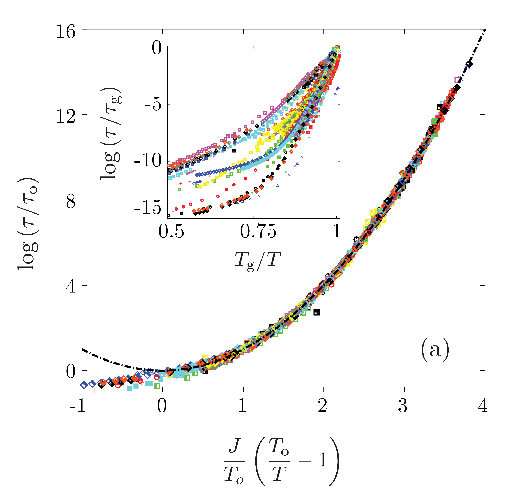
\includegraphics[height=0.675\textheight]{intro_glassy/newFigure1_v_9.eps}
    \caption{Transport and relaxation properties of 58 organic and inorganic liquids (Elmatad, Chandler, Garrahan, \textit{J. Phys. Chem. B},  2009)}
    
    
%    \label{fig:my_label}
%\end{figure}
\end{overprint}
\end{figure}

\end{column}

\begin{column}{0.5\linewidth}

\begin{enumerate}
    \item<2-> Glasses are formed from quenching a very viscous state of the liquid (\textbf{supercooled liquid})%Understanding the dynamics on the way to forming a solid glass 
    \item<6-> An \textbf{onset temperature} $T_\mathrm{o}$ delineates supercooled vs. high-temperature regime.
    \item<7-> Glassy dynamics is \textbf{ubiquitous}! 
    
    \only<7->{Ex: $m$-toluene, $n$-propanol}\only<8->{, metallic alloys, and colloidal suspensions}. 
\end{enumerate}

\onslide<9->{
\begin{block}{\centering \textbf{Motivating Question}}
What is the origin to the dramatic slowdown of (glassy) dynamics in supercooled liquids and its ``universal" nature?
\end{block}
}

\end{column}

\end{columns}
    
\end{frame}